\documentclass[aspectratio=169,12pt]{beamer}
\usepackage{amsmath}
\usepackage{amssymb}
\usepackage[most]{tcolorbox}
\usepackage{tikz}
\usepackage{graphicx}
\usepackage[sfdefault,lf]{FiraSans}
\renewcommand{\familydefault}{\sfdefault}
\setlength{\parindent}{0pt}
\everymath{\displaystyle}

\setbeamertemplate{navigation symbols}{}
\setbeamertemplate{footline}{}
\setbeamertemplate{headline}{}

\definecolor{mmpageWhite}{HTML}{FCFBF7}
\definecolor{mmtanSoft}{HTML}{F7F5EF}
\definecolor{mmgreenDeep}{HTML}{244B2C}
\definecolor{mmgreenLeaf}{HTML}{5D8A56}
\definecolor{mmgreenSoft}{HTML}{E4EFD9}
\definecolor{mmtext}{HTML}{163221}

\setbeamercolor{background canvas}{bg=mmpageWhite}
\setbeamercolor{normal text}{fg=mmtext,bg=mmpageWhite}

\newtcolorbox{MMProblemCard}[1][]{enhanced,breakable=false,colback=white,colframe=black,boxrule=1.5pt,arc=8pt,left=5pt,right=5pt,top=4pt,bottom=4pt,before skip=0pt,after skip=0pt,height=0.245\textheight,valign=top,#1}
\newcommand{\KoruIcon}{\raisebox{-0.2em}{
\includegraphics[height=1.05em]{../../SITE/header-logo.png}}}
\newcommand{\HoeIcon}{\raisebox{-0.2em}{
\includegraphics[height=1.05em]{../../SITE/hoe.png}}}
\newcommand{\ScaffoldIcons}[1]{\ifcase#1\or \HoeIcon\or \HoeIcon\hspace{0.22em}\KoruIcon\or \KoruIcon\hspace{0.22em}\KoruIcon\hspace{0.22em}\KoruIcon\fi}
\newcommand{\WorksheetTitle}[2]{%
  {\colorbox{mmtanSoft}{\parbox[c][2.0em][c]{0.975\linewidth}{%
    \hspace{0.25em}{\Large\bfseries\textcolor{mmgreenDeep}{#1}\hfill\ScaffoldIcons{#2}}}}
  \par\vspace{0.08em}{\color{mmgreenLeaf}\rule{\linewidth}{2.0pt}}\par\vspace{0.04em}}
}
\newcommand{\MMProblem}[2]{\begin{MMProblemCard}\raggedright\small\textbf{#1.} #2\par\end{MMProblemCard}}

\setbeamertemplate{background}{
 \begin{tikzpicture}[remember picture,overlay]
 \draw[black,line width=1.5pt,rounded corners=10pt]
 ([xshift=0.45cm,yshift=-0.45cm]current page.north west)
 rectangle
 ([xshift=-0.45cm,yshift=0.45cm]current page.south east);
 \end{tikzpicture}
}

% Default worksheet generation rules:
% use notes-style beamer pages
% use bordered cards for individual problems
% target 9 problems per frame in a 3x3 grid
% target 3 frames per scaffold by default where content allows

\begin{document}\begin{frame}[t]
\WorksheetTitle{Build Tasks}
\vspace{-0.18em}
\begin{columns}[T,onlytextwidth]
\begin{column}{0.32\textwidth}\MMProblem{1}{Find the perimeter.\\[0.4em]
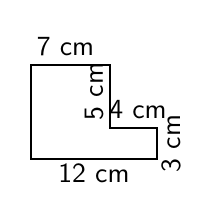
\begin{tikzpicture}[x=0.20cm,y=0.20cm,baseline=(current bounding box.center)]
  \draw[thick] (0,0)--(8,0)--(8,2)--(5,2)--(5,6)--(0,6)--cycle;
  \node at (4,-0.9) {12 cm};
  \node[rotate=90] at (8.9,1) {3 cm};
  \node at (6.8,3.2) {4 cm};
  \node[rotate=90] at (4.0,4.3) {5 cm};
  \node at (2.2,7.2) {7 cm};
\end{tikzpicture}}\end{column}
\begin{column}{0.32\textwidth}\MMProblem{2}{Find the perimeter.\\[0.4em]
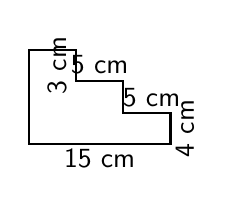
\begin{tikzpicture}[x=0.20cm,y=0.20cm,baseline=(current bounding box.center)]
  \draw[thick] (0,0)--(9,0)--(9,2)--(6,2)--(6,4)--(3,4)--(3,6)--(0,6)--cycle;
  \node at (4.5,-0.9) {15 cm};
  \node[rotate=90] at (9.9,1) {4 cm};
  \node at (7.8,3.0) {5 cm};
  \node at (4.5,5.1) {5 cm};
  \node[rotate=90] at (1.8,5) {3 cm};
\end{tikzpicture}}\end{column}
\begin{column}{0.32\textwidth}\MMProblem{3}{Find the perimeter.\\[0.4em]
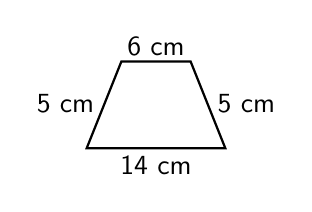
\begin{tikzpicture}[x=0.22cm,y=0.22cm,baseline=(current bounding box.center)]
  \draw[thick] (0,0)--(8,0)--(6,5)--(2,5)--cycle;
  \node at (4,-1.0) {14 cm};
  \node at (4,5.9) {6 cm};
  \node at (1.0,2.6) [left] {5 cm};
  \node at (7.0,2.6) [right] {5 cm};
\end{tikzpicture}}\end{column}
\end{columns}
\vspace{0.45em}
\begin{columns}[T,onlytextwidth]
\begin{column}{0.32\textwidth}\MMProblem{4}{Find the perimeter.\\[0.4em]
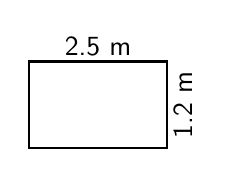
\begin{tikzpicture}[x=0.22cm,y=0.22cm,baseline=(current bounding box.center)]
  \draw[thick] (0,0) rectangle (8,5);
  \node at (4,5.9) {2.5 m};
  \node[rotate=90] at (8.9,2.5) {1.2 m};
\end{tikzpicture}}\end{column}
\begin{column}{0.32\textwidth}\MMProblem{5}{Find the perimeter.\\[0.4em]
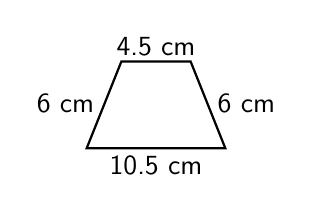
\begin{tikzpicture}[x=0.22cm,y=0.22cm,baseline=(current bounding box.center)]
  \draw[thick] (0,0)--(8,0)--(6,5)--(2,5)--cycle;
  \node at (4,-1.0) {10.5 cm};
  \node at (4,5.9) {4.5 cm};
  \node at (1.0,2.6) [left] {6 cm};
  \node at (7.0,2.6) [right] {6 cm};
\end{tikzpicture}}\end{column}
\begin{column}{0.32\textwidth}\MMProblem{6}{Find the perimeter.\\[0.4em]
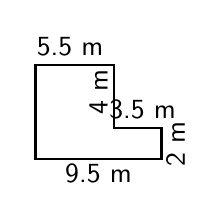
\begin{tikzpicture}[x=0.20cm,y=0.20cm,baseline=(current bounding box.center)]
  \draw[thick] (0,0)--(8,0)--(8,2)--(5,2)--(5,6)--(0,6)--cycle;
  \node at (4,-0.9) {9.5 m};
  \node[rotate=90] at (8.9,1) {2 m};
  \node at (6.8,3.2) {3.5 m};
  \node[rotate=90] at (4.0,4.3) {4 m};
  \node at (2.2,7.2) {5.5 m};
\end{tikzpicture}}\end{column}
\end{columns}
\vspace{0.45em}
\begin{columns}[T,onlytextwidth]
\begin{column}{0.32\textwidth}\MMProblem{7}{A rectangle has perimeter 38 cm and width 7 cm. Find its length.}\end{column}
\begin{column}{0.32\textwidth}\MMProblem{8}{A square garden has perimeter 18 m. How long is each side?}\end{column}
\begin{column}{0.32\textwidth}\MMProblem{9}{A triangle has sides 7.2 cm, 5.8 cm and 6.5 cm. Find its perimeter.}\end{column}
\end{columns}
\end{frame}
\begin{frame}[t]
\WorksheetTitle{Build Tasks}
\vspace{-0.18em}
\begin{columns}[T,onlytextwidth]
\begin{column}{0.32\textwidth}\MMProblem{1}{A shape has side lengths 4 cm, 6 cm, 3 cm, 5 cm, 2 cm and 8 cm. Find its perimeter.}\end{column}
\begin{column}{0.32\textwidth}\MMProblem{2}{Jordan says a \mbox{$9$} cm by \mbox{$4$} cm rectangle has perimeter \mbox{$13$} cm. Explain the mistake and give the correct perimeter.}\end{column}
\begin{column}{0.32\textwidth}\MMProblem{3}{A rectangle is twice as long as it is wide. Its perimeter is 30 cm. Find the length and width.}\end{column}
\end{columns}
\vspace{0.45em}
\begin{columns}[T,onlytextwidth]
\begin{column}{0.32\textwidth}\MMProblem{4}{The perimeter of an equilateral triangle is 27 cm. Find one side length.}\end{column}
\begin{column}{0.32\textwidth}\MMProblem{5}{A rectangle is 13 m long and 4 m wide. Find its perimeter.}\end{column}
\begin{column}{0.32\textwidth}\MMProblem{6}{A regular pentagon has side length 6 cm. Find its perimeter.}\end{column}
\end{columns}
\vspace{0.45em}
\begin{columns}[T,onlytextwidth]
\begin{column}{0.32\textwidth}\MMProblem{7}{The perimeter of a square is 44 mm. Find one side length.}\end{column}
\begin{column}{0.32\textwidth}\MMProblem{8}{}\end{column}
\begin{column}{0.32\textwidth}\MMProblem{9}{}\end{column}
\end{columns}
\end{frame}
\end{document}
